\begin{figure}
    \centering
    \begin{subfigure}[b]{0.35\linewidth}
        \centering
        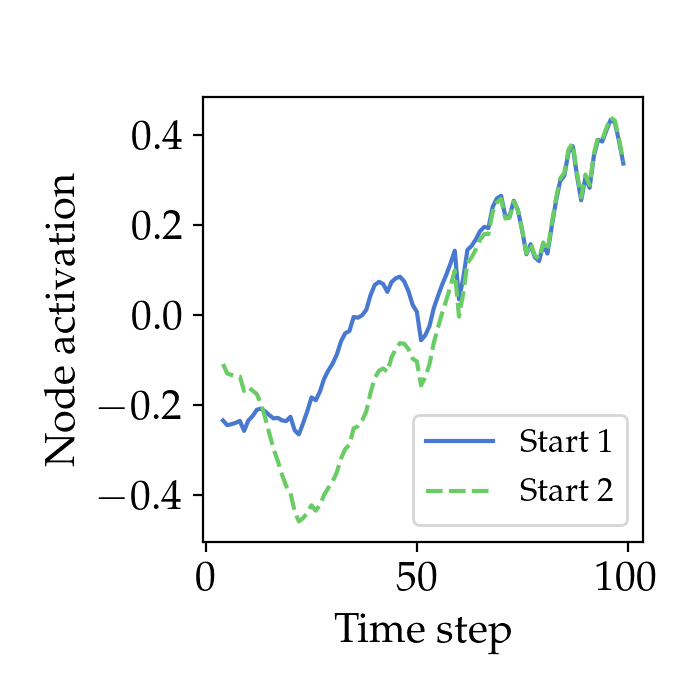
\includegraphics[height=5.7cm,keepaspectratio]{img/explainer_fading_mem.png}
        \caption{ }
        \label{fig:fading_mem_principle}
    \end{subfigure}
    \hfill
    \begin{subfigure}[b]{0.62\linewidth}
        \centering
        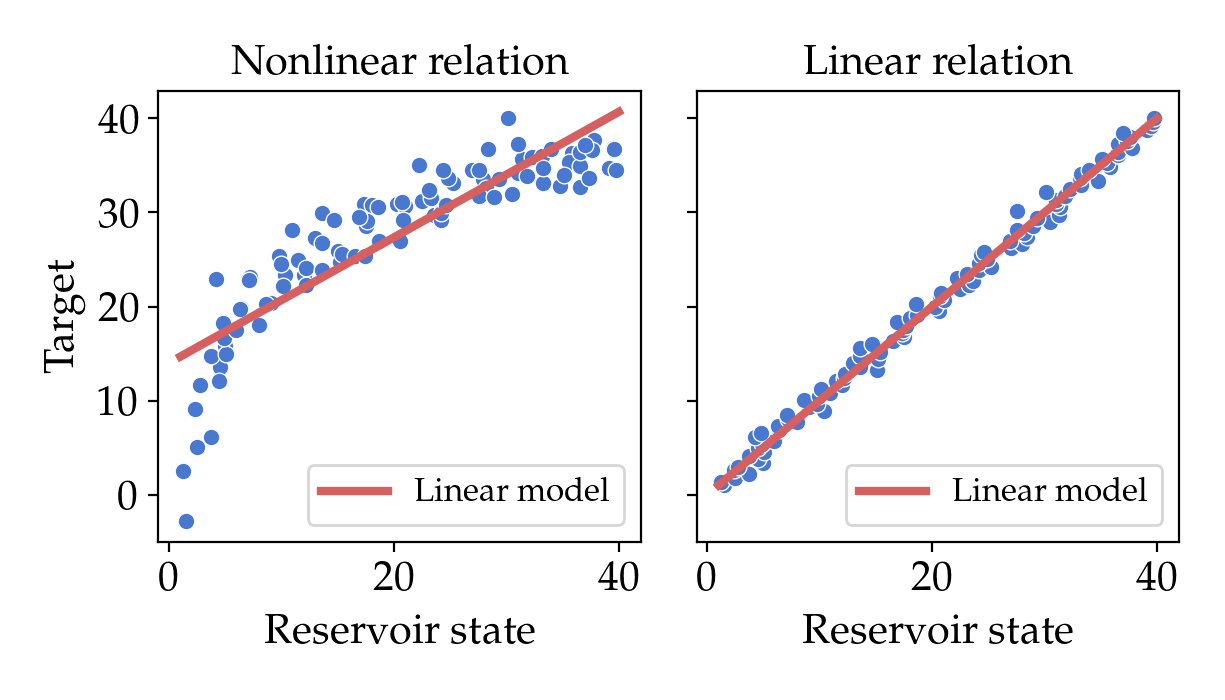
\includegraphics[height=5.7cm,keepaspectratio]{img/explainer_input_sep.png}
        \caption{ }
        \label{fig:input_sep_principle}
    \end{subfigure}
    \caption[Demonstration of the Echo State Property and illustration of linear input separation.]{
        Demonstration of the Echo State Property and illustration of linear input separation.
        (\subref{fig:fading_mem_principle}) Demonstration of the \acrlong{esp} in an ESN with 100 nodes, leak rate 0.16 and spectral radius 1.25. The ESN is subjected to the same input sequence, with two different initial state vectors. The plot shows the activation value of the same node through time.
        (\subref{fig:input_sep_principle}) Example of linear input separation between a target task and the reservoir state. The left plot shows a nonlinear relation (in this case, logarithmic). The right plot shows a linear relation. The red line shows a linear regression model fitted to the data.
    }
    \label{fig:prc_principles}
\end{figure}

